\chapter{仙人掌图表示法标准化算法}

仙人掌图表示法保留了原图所有的最小割信息,
因此如果能差分隐私地输出图的仙人掌图表示法,
那么也就完成了差分隐私下近似最小割的求解。
然而,Dinitz的论文\cite{dinitz1976structure}中提供的仙人掌图表示法定义
存在一定局限性,为隐私化带来了障碍。
本章将从仙人掌图表示法的定义出发,
给出一个仙人掌图表示法的标准化算法,
该算法是差分隐私下仙人掌图表示求解算法的前置基础。
同时,借助对仙人掌图表示法的分析,
本文也将在后续章节中完成对最小割性质的分析。

\section{Dinitz仙人掌图表示法简述}

仙人掌图表示法的标准化算法,是在Dinitz仙人掌图表示法\cite{dinitz1976structure}的基础上完成设计的。
本节将简述仙人掌图表示法的构建与图本身的关联。
根据定义\ref{cactus},给定任意带权图$G$,
存在仙人掌图$\Gamma$和映射$\varphi$作为其仙人掌图表示法。

仙人掌图表示法能够表示的割分为两类,其对应原图$G$中的$p$割与$t$割,
这种对应得益于割本身具有的次模性。
此处将首先介绍次模性和其推论,它们是后文分析中的重要工具。


\begin{lemma}[割的次模性]\cite{cunningham1985minimum}
  给定图$G=(V,E)$和图的两个割$\Delta(X),\Delta(Y)$,有
  \begin{equation}
    w(X)+w(Y)\geq w(X\cup Y)+w(X\cap Y)
  \end{equation}
\end{lemma}

\begin{lemma}[次模性推论]
  给定图$G$和图中两个相交的割$\Delta(X),\Delta(Y)$,则有如下结论:
  \begin{itemize}
    \item $w(X\cap Y)=\Phi_G$
    \item $w(X\cap Y,X\cap (V\backslash Y))=\frac {\Phi_G}2$
    \item $w(X\cap Y,(V\backslash X)\cap (V\backslash Y))=0$
  \end{itemize}
\end{lemma}
\begin{proof}
  首先证明第一条结论。根据割的次模性,可以得到
  \begin{equation}
    2\Phi_G\leq w(X\cup Y)+w(X\cap Y)\leq w(X)+w(Y) = 2\Phi_G
  \end{equation}
  因此,$w(X\cup Y)=w(X\cap Y)=\Phi_G$。

  接下来证明第二条结论。根据第一条结论的对称性,
  $w(X\cap Y)=w(X\cap (V\backslash Y))=\Phi_G$;由于$\Delta(Y)$是最小割,所以$w(Y)=\Phi_G$。
  根据$w$的定义,有
  \begin{equation}
    w(X\cap Y)+w(X\cap (V\backslash Y))=w(Y)+2w(X\cap Y,X\cap (V\backslash Y))
  \end{equation}
  因此,$w(X\cap Y,X\cap (V\backslash Y))=\frac {\Phi_G}2$。

  最后证明第三条结论。根据第二条结论的对称性$ w(X\cap Y,X\cap (V\backslash Y))+w(X\cap Y,(V\backslash X)\cap Y)=\frac{\Phi_G}2$。
  根据$w$的定义,有
  \begin{equation}
    w(X\cap Y,X\cap (V\backslash Y))+w(X\cap Y,(V\backslash X)\cap Y)+w(X\cap Y,(V\backslash X)\cap (V\backslash Y))=w(X\cap Y)=\Phi_G
  \end{equation}
  因此,$w(X\cap Y,(V\backslash X)\cap (V\backslash Y))=0$。
\end{proof}

接下来将给出若干定义来解释$p$割和$t$割这两个概念。
在仙人掌图表示法的最初构造方法中,求解$p$割与$t$割是流程的第一步。

\begin{definition}[割的平行与相交]
  设 $R = (X, Y)$和 $R' = (X', Y')$是图中的不同割,它们的相对位置存在两种可能情况:
  \begin{itemize}
    \item 集合 $X \cap X'$、 $X \cap Y'$、 $Y \cap X'$、 $Y \cap Y'$均非空;
    \item 这些集合中存在空集。
  \end{itemize}
  在第一种情况下,割 $R$和 $R'$被称为相交的一对割,在第二种情况下,它们被称为平行的一对割。
\end{definition}
\begin{figure}[htb]
  \centering
  \subfloat[相交的一对割]{
    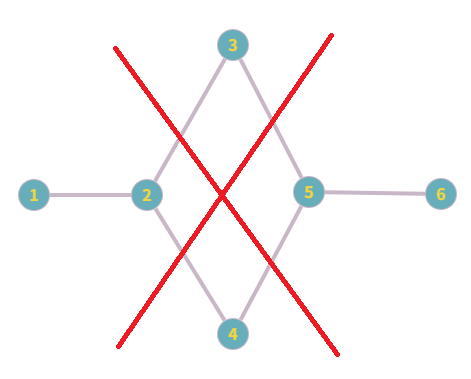
\includegraphics[height=5cm]{figures/graph006.png}}\hspace{4em}
  \subfloat[平行的一对割]{
    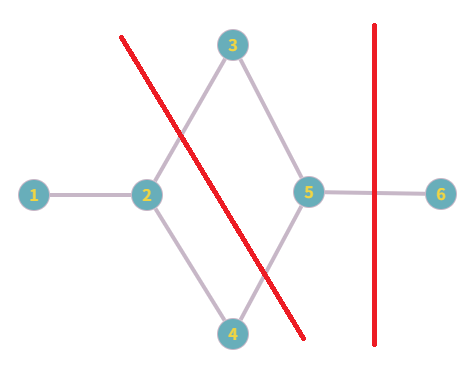
\includegraphics[height=5cm]{figures/graph007.png}}
  \caption{割的平行与相交例}
  \label{crosscut}
\end{figure}
如图\ref{crosscut}所示,灰色的直线代表图中节点的连边,红色直线代表割,
左右两图分别对应相交和平行的割的例子。

\begin{definition}[最小割图]
  给定图$G$和其最小割集$R^*(G)$,最小割图按如下方式生成:
  \begin{itemize}
    \item 对于每个最小割$r\in R^*(G)$,在最小割图中新建一个与之相对应的点。
    \item 若两个最小割$r_1,r_2$相交,则在最小割图中对应的点之间连一条边。
  \end{itemize}
\end{definition}

\begin{definition}[$p$割与$t$割]
  如果图$G$的一个最小割$R$与其他任何最小割都平行,就称它为$p$割;否则,称它为$t$割。
\end{definition}
\begin{figure}[htb]
  \centering
    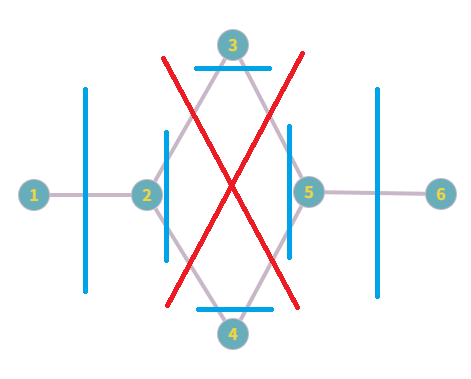
\includegraphics[height=5cm]{figures/graph008.png}
  \caption{$p$割和$t$割例}
  \label{ptcut}
\end{figure}
如图\ref{ptcut}所示,
蓝色直线为图中的$p$割,
红色直线为图中的$t$割。

仙人掌图表示法的构造分为两步,
第一步是构建能表示所有$p$割的树表示法,
第二步是用环状结构图替代$p$束顶点。

\begin{definition}[处于两个$p$割之间的点和割]
  给定两个$p$割$R=(X,Y)$和$R'=(X',Y')$,
  不妨假设$X\cap Y'=\emptyset$。
  称点$v$处于$R$和$R'$之间当且仅当$v\in X'\cap Y$。
  称割$R''=(X'',Y'')$处于$R$和$R'$之间当且仅当 $X\subset X''$且$Y'\subset Y''$。
\end{definition}


\begin{figure}[htb]
  \centering
    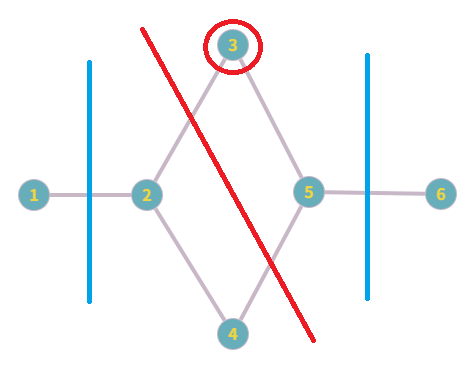
\includegraphics[height=5cm]{figures/graph009.png}
  \caption{处于两个$p$割之间的点和割例}
  \label{between}
\end{figure}
如图\ref{between}所示,
红色圈中顶点以及红色直线代表的割处于两个蓝色直线表示的$p$割之间。

\begin{definition}[相邻的$p$割]
  给定两个$p$割$R$和$R'$,称它们相邻当且仅当不存在处于它们之间的$p$割。
\end{definition}

对于一个$p$割$R=(X,V\backslash X)$,记$S(X)$为所有与$R$相邻且分隔开$X$中顶点的$p$割的集合。
需要注意,$S(X)$与$S(V\backslash X)$对应该$p$割的两侧。

\begin{definition}[$p$束]
  给定一个$p$割集合$S$,称其为$p$束当且仅当
  存在一个$p$割$R=(X,V\backslash X)$满足$S=S(X)\cup \{R\}$。
  特别的,当$S$中仅包含一个$p$割$R=(X,V\backslash X)$时,该$p$束为叶$p$束,用$S_X$表示,记该$p$束由$R$的$X$一侧得到。
\end{definition}
图的所有$p$束可以通过枚举所有$p$割以及其两侧得到,也就是说,图的$p$束集合是有限且唯一确定的。

\begin{definition}[$p$束内部的顶点和$t$割]
  顶点$v$属于$p$束$S$当且仅当对于任意一对$p$束中的$p$割
  都满足该顶点在这两个割之间,
  此类顶点的集合记作$V(S)$。
  $t$割属于$p$束$S$当且仅当对于任意一对$p$束中的$p$割
  都满足该$t$割在这两个割之间。
  特别的,对于叶$p$束$S_X$,顶点$v$属于$S$当且仅当$v\in X$,$t$割不会属于叶$p$束。
\end{definition}
需要特别说明,根据割的次模性推论,
一组在最小割图中连通的$t$割对应至少$4$个$p$割,
因此若$t$割属于叶$p$束$S_X$,则与$S_X$只包含一个$p$割这一结论矛盾。
\begin{definition}[相邻的$p$束]
  两个$p$束$S,S'$相邻当且仅当$S\cap S'$非空。
\end{definition}
当$S,S'$相邻时,$S,S'$分别位于$R$的两侧,因此$S\cap S'$中的元素是唯一的。
在这些概念的基础上,Dinitz等人提出了可以表示所有$p$割的树表示法。

\begin{theorem}[树表示法]\cite{dinitz1976structure}
  \label{treerepresentation}
  给定带权图$G$,存在一个棵树$\Lambda$和映射$\phi:V_G\rightarrow V_\Lambda$,满足:
    \begin{itemize}
        \item 对于点$v_1,v_2\in V_G$,$\phi(v_1)=\phi(v_2)$当且仅当图$G$不存在$p$割$R=(V_1,V_2)$使得$v_1\in V_1,v_2\in V_2$;
        \item 图$G$的最小割$R=(V_1,V_2)$与图$\Lambda$的最小割$(\phi(V_1),V_\Lambda\backslash\phi(V_1))$一一对应。
    \end{itemize}
\end{theorem}

\begin{theorem}[树表示法的性质]\cite{dinitz1976structure}
  \label{treerepresentation2}
  图$G$的树表示法$\Lambda$有以下两个性质:
  \begin{itemize}
    \item $\Lambda$上每一条边的边权都等于最小割的割值。
    \item $\Lambda$中的点与$p$束一一对应,边与$p$束的相邻关系一一对应。
  \end{itemize}
\end{theorem}

为了辅助仙人掌图表示法的标准化算法,接下来的引理将说明树表示法的唯一性。

\begin{lemma}[树表示法的唯一性]
  \label{treeunique}
  给定带权图$G$,其树表示法$(\Lambda,\phi)$唯一。
\end{lemma}
\begin{proof}
  使用反证法,不妨假设图$G$有两个不相同的树表示法$(\Lambda,\phi)$和$(\Lambda',\phi')$。
  首先证明$\phi=\phi'$。根据定理\ref{treerepresentation}的第一条性质,若存在$v_1,v_2\in V_G$满足$\phi(v_1)=\phi(v_2)$但$\phi(v_1)\neq\phi(v_2)$,
  则将两点分隔开的$p$割的存在性出现矛盾。

  接下来证明$\Lambda=\Lambda'$。
  图$G$的$p$束集合有限且唯一确定,
  定理\ref{treerepresentation2}表明树表示法的树结构$\Lambda$中,
  顶点与$G$的$p$束一一对应,边与$p$束的相邻关系一一对应。
\end{proof}

在树表示法中,顶点与$p$束一一对应,每个$t$割都唯一属于一个$p$束。
接下来将分析$t$割在仙人掌图表示法中的表示形式。

\begin{definition}[原子]
  给定图$G=(V,E)$和$G$中割的集合$\mathcal{C}$。$\mathcal{C}$的原子是一个$V$的划分$P$的所有划分块,其中$P$满足
  \begin{itemize}
    \item 对于任意割$(X,V\backslash X)\in \mathcal{C}$以及任意原子$A\in P$,满足$A\subseteq X$或$A\subseteq V\backslash X$。
    \item $P$是满足条件的最粗划分,也就是说对于任何满足条件的划分$P'$,都有$P'\preceq P$。
  \end{itemize}
\end{definition}

给定的一组割会将图的点集划分成若干块,每个划分块对应一个原子。

\begin{theorem}[最小割和$p$割对应的原子集等价]\cite{dinitz1976structure}
  给定图$G$,由所有最小割构成的割集得到的原子集和由所有$p$割构成的割集得到的原子集等价。
\end{theorem}

这一定理表明,一个$p$束内不会同时包含顶点和$t$割。

\begin{definition}[$p$束结构图$G_S$]
定义$G_S$为图$G$中$p$束$S$的结构图,其生成方式如下:
\begin{itemize}
  \item 将$G_S$初始化为$G$。
  \item 枚举$S$中的$p$割$R$,并对被该割与$S$分隔开的点集执行点收缩(同时记收缩得到的点为$x_R$)。
\end{itemize}
\begin{definition}[$\hat c$环]
  所有边的权重都为 $\hat{c}/2$的环被称为 $\hat{c}$环。 
\end{definition}
\end{definition}
\begin{theorem}[含$t$割的$p$束的结构图为环]\cite{dinitz1976structure}
  \label{ring}
  如果一个 $p$ 束 $S$存在内部的$t$割,
  那么图 $G_S$是以顶点 $x_R$( $R\in S$)构成的 $\hat{\Phi_G}$环 。
\end{theorem}
定理\ref{ring}说明了当$p$束$S$内存在$t$割的情况,其核心结论主要有两点。第一个结论是当$S$内存在$t$割时,
则$V(S)=\emptyset$,这对应了$\hat{\Phi_G}$环仅由$x_R$即$S$外部的顶点构成这一结果;
第二个结论是$S$内的$t$割恰好是将环分成两部分的割(每一部分至少包含两个顶点),且这些$t$割在最小割图中恰好构成一个联通块。

Dinitz等人在树表示法中用环替换含$t$割的$p$束对应的顶点,得到了仙人掌图表示法的构造算法。
因此,在仙人掌图表示法中,
非环边代表$p$割,$t$割仅由环边二元组表示。



\section{仙人掌图表示法的不唯一性}

仙人掌图表示法由仙人掌图$\Gamma$和映射$\varphi$共同构成。
首先,本节将定义仙人掌图表示法对应的割集,
这一概念展示了,在已知仙人掌图$\Gamma$和映射$\varphi$的情况下,
如何还原出原图的最小割集合。

还原的过程需要用到仙人掌图表示法中映射$\varphi$的逆映射$\varphi^{-1}$,
该逆映射是从$V_\Gamma$到$\mathcal{P}(V_G)$的映射。
分析$\varphi$的性质可得,$\Gamma$中的点对应着$G$中的$0$个、$1$个或多个顶点。
下面将给出仙人掌图表示法对应割集的表示形式,
并由此定义仙人掌图表示法的等价性。

\begin{definition}
  \label{cactusequal}
  给定点集$V$,仙人掌图表示法由仙人掌图$\Gamma$和映射$\varphi:V\rightarrow V_\Gamma$构成,
  其对应的割集为
  \begin{equation}
    CutSet(\Gamma,\varphi)=\{(X,Y)\in R^*_{\Gamma}|(\bigcup_{x\in X}\varphi^{-1}(x),\bigcup_{y\in Y}\varphi^{-1}(y))\}
  \end{equation}
  两个仙人掌图表示法$(\Gamma,\varphi),(\Gamma',\varphi')$等价当且仅当$CutSet(\Gamma,\varphi)=CutSet(\Gamma',\varphi')$。
\end{definition}

一个仙人掌图表示法唯一对应了原图的最小割集,
但原图的最小割集可能对应多个仙人掌图表示法。

\begin{lemma}
  \label{cactusnonunique}
  图的仙人掌图表示法不具有唯一性。
\end{lemma}
\begin{proof}
  证明将通过给出一个图$G$以及其两个不相同的仙人掌图表示法$(\Gamma,\varphi),(\Gamma',\varphi')$的构造来完成。
  \begin{figure}[htb]
    \centering
    \subfloat[图$G$]{
      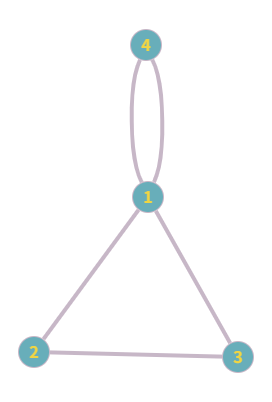
\includegraphics[height=5cm]{figures/graph003.png}}\hspace{4em}
    \subfloat[图$\Gamma$]{
        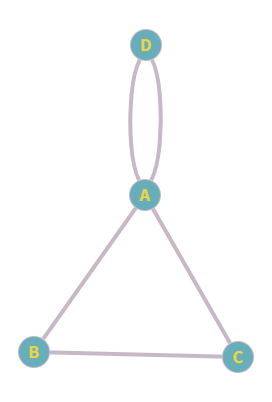
\includegraphics[height=5cm]{figures/graph004.png}}\hspace{4em}
    \subfloat[图$\Gamma'$]{
      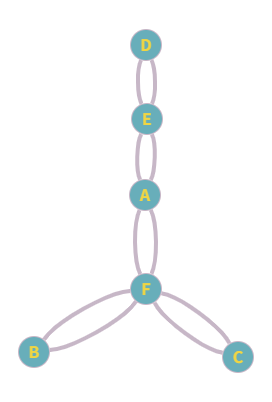
\includegraphics[height=5cm]{figures/graph005.png}}
    \caption{同一个图的两种仙人掌图表示法}
    \label{diffent_cac}
\end{figure}

图$\ref{diffent_cac}$给出了$G,\Gamma,\Gamma'$的结构,
其中$n=4$。仙人掌图表示法的映射部分$\varphi,\varphi'$取值为
\begin{equation}
  \varphi=\varphi'=\{(1,A),(2,B),(3,C),(4,D)\}
\end{equation}

在该构造下,图$G$的最小割集为
\begin{equation}
\{(\{1,4\},\{2,3\}),(\{1,2,4\},\{3\}),(\{1,3,4\},\{2\}),(\{1,2,3\},\{4\})\}
\end{equation}
仙人掌图表示法$(\Gamma,\varphi)$中,$\Gamma$与$G$结构相同,
因此最小割一一对应。
仙人掌图表示法$(\Gamma',\varphi')$进行了两个改动:
第一个改动是通过加入节点$F$,使$A,B,C$构成的三元环变成三个二元环,
三元环所表示的最小割分别转而由这三个二元环所表示,所以该改动不影响割集,
以割$(\{1,3,4\},\{2\})$为例,其由$\Gamma$中的三元环边$(A,B),(B,C)$共同表示,
而到了$\Gamma'$中,其转而由两条$(B,F)$边构成的二元环表示;
第二个改动是在$A$和$D$之间加入$E$,这使得$\Gamma'$中的最小割数量增加,
即$(\{A,B,C,F\},\{D\})$扩展成了$(\{A,B,C,F\},\{D,E\})$和$(\{A,B,C,E,F\},\{D\})$两个最小割,
然而由于$\varphi^{-1}(E)=\emptyset$,因此这两个$\Gamma'$中的割对应$G$的同一个割,改动不影响割集。
综上,$(\Gamma,\varphi),(\Gamma',\varphi')$都是$G$的仙人掌图表示法,图的仙人掌图表示法不具有唯一性。
\end{proof}

图的最小割集是唯一的,
所以同一个图的仙人掌图表示法对应的割集相同,即仙人掌图表示法等价。
也就是说,图的仙人掌图表示法不具有唯一性,但具有等价性。

\section{标准化仙人掌图表示法}

本节将设计仙人掌图表示法等价类的标准元,
并给出仙人掌图表示法的标准化算法。
仙人掌图表示法的生成算法结束后,
将输出通过标准化算法转化为等价类的标准元,
那么就可以确保对于相同的原图,
可以得到具有唯一性的仙人掌图表示法。

对于最小割集相同的边相邻图,
常规算法可能受边集差异的影响,
得到两个等价但不相等的仙人掌图表示法。
在差分隐私场景下,
算法需要确保等价的仙人掌图表示法被判定为相同,
本节提出的标准化算法可以解决这一问题。

本节中仙人掌图表示法的标准化共分为两部分:
第一部分通过构造来定义仙人掌图表示法的标准元,
第二部分给出将仙人掌图表示法转化为其标准元的高效算法。

根据引理\ref{treeunique},树表示法$\Lambda$可以表示所有$p$割,
且其形态具有唯一性。
根据定理\ref{ring},$p$束的结构图可以表示该$p$束的所有$t$割且其形态具有唯一性。
因此,如果将树表示法和每个$p$束的结构图
用一种确定性方法进行合成,
得到的仙人掌图表示法也是唯一的,且恰好能表示所有的最小割。
本文设计了一种能使合成产生的仙人掌图表示法拥有较好性质的方法,
并将用该方法生成的图设置为该仙人掌图表示法的标准元。
由图$G$生成仙人掌图表示法标准元的具体算法$ALG_{gen}$在算法\ref{alg:gen}中给出,
同时,称$ALG_{gen}(G)$为图$G$的标准仙人掌图表示法。

\begin{algorithm}
  \caption{图$G$的仙人掌图表示法构造算法$ALG_{gen}$}
  \label{alg:gen}
  \begin{algorithmic}[1] % [1] 表示从第1行开始编号
  \Statex 输入:图$G$
  \Statex 输出:仙人掌图表示法$(\Gamma,\varphi)$
  \State 计算图$G$的所有$p$割,$t$割。
  \State 计算图$G$中的所有$p$束。
  \State 为每个$p$束$S$新建一个$\Gamma$中的点$v_S$,并更新$S$内的原图顶点到$v_S$的映射$\varphi$。
  \State 若两个$p$束$S,S'$相邻,则为其在$\Gamma$中的点$v_S,v_{S'}$连一条边,得到图$G$的树表示法。
  \State 若$p$束$S$中有$t$割,则将$v_S$替换为$G_S$。
  若一条边连向$v_S$,设该边代表的$p$割为$R$,
  则请其重新连向$G_S$中的点$x_R$。
  \State \Return $(\Gamma,\varphi)$
  \end{algorithmic}
\end{algorithm}

接下来的定理将说明,若两个图的仙人掌图表示法等价,则其标准仙人掌图表示法也相同。

\begin{theorem}
  给定图$G,G'$,已知它们的仙人掌图表示法分别为$(\Gamma,\varphi)$和$(\Gamma',\varphi')$。
  若$(\Gamma,\varphi)$和$(\Gamma',\varphi')$等价,则$ALG_{gen}(G)=ALG_{gen}(G')$。
\end{theorem}

\begin{proof}
  条件中提到,$(\Gamma,\varphi)$和$(\Gamma',\varphi')$等价,根据定义\ref{cactusequal},有 $CutSet(\Gamma,\varphi)=CutSet(\Gamma',\varphi')$。
  由仙人掌图表示法的定义,
  $CutSet(\Gamma,\varphi)$和$CutSet(\Gamma',\varphi')$分别对应$G$的最小割集和$G'$的最小割集。
  $ALG_{gen}(G)$的步骤仅用到了$G$的最小割集的信息,
  因此若最小割集相同,算法输出也相同,即$ALG_{gen}(G)=ALG_{gen}(G')$。
\end{proof}

对于一个仙人掌图表示法,其标准元为其原图$G$的标准仙人掌图表示法$ALG_{gen}(G)$。
算法\ref{alg:gen}以构造的形式定义了标准仙人掌图表示法及标准元,
但不能直接用于标准元的求解中。
主要问题有两方面,一方面是其用到了原图$G$的信息,
因此在仅有仙人掌图表示法时不能直接使用;
另一方面是,$p$割、$t$割、$p$束的计算复杂度较高,易成为算法的效率瓶颈。

因此,本节接下来将给出一仙人掌图表示法的标准化算法$ALG_{std}$,
其可以将现有工作生成的仙人掌图表示法直接转化为等价类内的标准元,
而不需要获取原图信息。
与此同时,
$ALG_{std}$高效利用了输入仙人掌图表示法的信息,
复杂度相比$ALG_{gen}$显著降低。其具体实现如算法\ref{algstd}所示。


\begin{algorithm}
  \caption{仙人掌图表示法标准化算法$ALG_{std}$}
  \label{algstd}
  \begin{algorithmic}[1] % [1] 表示从第1行开始编号
  \Statex 输入:仙人掌图表示法$(\Gamma,\varphi)$
  \Statex 输出:标准仙人掌图表示法$(\Gamma',\varphi')$
  \State 设仙人掌图表示法$(\Gamma,\varphi)$的最小割的割值为$c$;
  \State 对所有二元环,将两条环边合并为一条边,边权求和;\Comment{等价转换}
  \For {$\Gamma$中的简单环$C$}
      \For {$C$中的节点$k$}
          \State 在$\Gamma$中新建顶点$k',k''$来替换$k$,\Comment{分离简单环中的$p$割}
          \State 令$\varphi^{-1}(k'')=\varphi^{-1}(k),\varphi^{-1}(k')=\emptyset$,
          \State 在$k',k''$之间连一条边权为$c$的边;
          \For {与$k$相连的边$e$}\Comment{边的重连}
            \If{$e$是环$C$上的边}
                \State 将$e$的$k$一端替换成$k'$;
            \ElsIf{$e$不是环$C$上的边}
                \State 将$e$的$k$一端替换成$k''$;
            \EndIf
          \EndFor
      \EndFor
  \EndFor
  \State 对$\Gamma$中的所有三元环执行点收缩;\Comment{$p$割已被分离,三元环为冗余结构}
  \For {$\Gamma$中度数为$2$的点$v$}\Comment{删除冗余空节点}
      \If{若$v$不处于任何一个简单环上且$\varphi^{-1}(v)=\emptyset$}
          \State 找到与$v$相连的边$(v,u_1),(v,u_2)$;
          \State 删除点$v$以及与其相连的边;
          \State 加入边$(u_1,u_2)$;
      \EndIf
  \EndFor
  \State \Return $(\Gamma',\varphi')$
  \end{algorithmic}
\end{algorithm}

回顾引理\ref{cactusnonunique}中给出的仙人掌图表示法不唯一性的例子,
可知产生的差异有三元环的两种表达形式,以及冗余链等情况。
算法\ref{algstd}通过分离环上的$p$割以及冗余结构的处理,确保了到标准仙人掌图表示法的转换。

\begin{theorem}
  给定图$G$和其仙人掌图表示法$(\Gamma,\varphi)$,则$ALG_{std}((\Gamma,\varphi))=ALG_{gen}(G)$
\end{theorem}

\begin{proof}
  首先,需要证明$ALG_{std}((\Gamma,\varphi))$算法得到的环与$ALG_{gen}(G)$的环一一对应。
  在仙人掌图表示法中,非环边代表的最小割一定是$p$割,
  环中的一对边代表的最小割可能是$p$割也可能是$t$割。
  根据算法\ref{alg:gen},
  $ALG_{gen}(G)$的$p$割全部对应了树表示法的边,
  环仅用于表示$t$割,也就是说,环上相邻边构成的$p$割不予考虑。
  对于一个$ALG_{gen}(G)$中的简单环$C$,
  其表示的$t$割在最小割图中恰好构成一个连通块,
  因此这些割在$(\Gamma,\varphi)$中一定对应一个相同大小的环$C'$。
  需要特别说明的是,对于这个仙人掌图表示$(\Gamma,\varphi)$中的环$C'$,
  环上相邻的两条边表示一个$p$割,这些$p$割在算法中通过$(k',k'')$这条非环边重新表示,
  因此此时环不再具有表示$p$割的作用。
  若环$C'$不表示任何$t$割,那么其一定是一个二元环或三元环,
  同时由于其不具有表示$p$割的作用,这些环是冗余结构,在算法中被消除。
  综上,$ALG_{std}((\Gamma,\varphi))$算法得到的环与$ALG_{gen}(G)$的环一一对应。

  接下来证明将所有环缩成点后,
  $ALG_{std}((\Gamma,\varphi))$的树结构和$ALG_{gen}(G)$的树结构相同。
  $(\Gamma,\varphi)$的$p$割由非环边和环共同表示,而在处理环的过程中,
  所有环表示的$p$割转而以$(k',k'')$的非环边形式表示。因此,处理完环之后,$(\Gamma,\varphi)$的树结构和$ALG_{gen}(G)$
  都能表示所有$p$割。此时,$(\Gamma,\varphi)$的树结构表示了所有$p$割,但不一定是树表示法,
  因为树表示法的边与$p$割一一对应,但是树结构可以存在多条边对应同一个$p$割的情况。
  代表同一个$p$割的两条边之间的树上路径的点$v$都满足$\varphi^{-1}=\emptyset$,
  因此,$ALG_{std}$可以通过收缩所有这样的冗余顶点,将树结构转化为树表示法。
  根据定理\ref{treerepresentation},树表示法具有唯一性。
  综上, $ALG_{std}((\Gamma,\varphi))$的树结构和$ALG_{gen}(G)$的树结构相同。

  结合以上两个结果,可以得出$ALG_{std}((\Gamma,\varphi))=ALG_{gen}(G)$。
\end{proof}